\chapter{Implementation of the Linux scheduler}
\label{chap:implementation}

\section{Structs and their role}

\paragraph{task\_struct}
As mentioned in chapter \ref{ch:introduction}, each task in the system is represented \newline by a \verb|task_struct|, which contains all the information about it. Here we list some of the fields used by the scheduler, and then cover them in detail.
\begin{itemize}
    \item \verb|thread_info|. This struct is architecture dependant and can contain various fields. The most important for the scheduler is the \verb|flags| field. These flags are used to keep track of requests or signals from and for the task. \verb|TIF_SIGPENDING| means that the process has pending signals, \verb|TIF_MEMDIE| means that the process is being killed to reclaim memory. In particulare, there are two flags that are crucial for the scheduler: \verb|TIF_NEED_RESCHED| and \verb|TIF_POLLING_NRFLAG|. The first indicates that scheduling must be performed, and the second that the idle process is polling the \verb|TIF_NEED_RESCHED| flag.
    %from cesati's book
    \item \verb|state|. A long that represents the state of the task: -1 unrunnable, 0 runnable, $>0$ stopped. 
    \item \verb|on_rq|. Indicates if the process is on the runqueue.
    \item \verb|static_prio| and \verb|normal_prio|. The first is the priority used for real-time scheduling policies. If the task is scheduled under one of the normal scheduling policies \verb|static_prio| is set to zero and \verb|normal_prio| is used. This number is an internal representation used in the kernel, different from the priority value shown in user space.
    \item \verb|sched_entity|. This struct contains all the other information needed by the scheduler.
    \item Pointer to \verb|sched_class|. The scheduling class discussed in chapter \ref{ch:sched}. Contains a circular list of all scheduling classes.
    \item Pointer to \verb|mm_struct|. This struct represents the slice of virtual memory used by the process. Here, ``\verb|mm|'' stands for \textit{memory management}.
\end{itemize}

\paragraph{thread\_info}
\label{sec:thread_info}
This structure is very small and contains only basic information useful for scheduling, and each process has its own \verb|thread_info|. In figure \ref{img:stack} from chapter \ref{ch:introduction} it is shown that this struct is located at the bottom of kernel stacks. The small size of this struct is due to the fact that it has to fit in the small kernel stacks while not occupying too much space. Today, the implementation of \verb|thread_info| has changed: it is now embedded directly in \verb|task_struct|. 

\begin{code}
struct task_struct {
#ifdef CONFIG_THREAD_INFO_IN_TASK
	/*
	 * For reasons of header soup (see current_thread_info()), this
	 * must be the first element of task_struct.
	 */
	struct thread_info  thread_info;
#endif
// ...
\end{code}
With the previous implementation, \verb|thread_info| and \verb|task_struct| referenced each other through pointers. As shown in this code, if \verb|CONFIG_THREAD_INFO_IN_TASK| is defined, the field is not a pointer. With this new implementation, \verb|thread_info| is not located in the kernel stack. In order to access it, a pointer to the current task's \verb|thread_info| is saved, and its \verb|task_struct| can be accessed with the ``\verb|container_of()| trick'' discussed in chapter \ref{ch:introduction}. 

The implementation of this struct is very architecture dependent. This one is specific to x86:
\begin{code}
struct thread_info {
	unsigned long   flags;  /* low level flags */
	u32 status;             /* thread synchronous flags */
};
\end{code}
The flags field is crucial, because it is here that the \verb|TIF_NEED_RESCHED| flag is set, allowing the scheduler to be invoked. In practice, there are pieces of code that are executed each time a task enters/exits kernel space. In particular, when returning to user space, each task will execute the \textit{userspace return path}, defined in assembly in \verb|./arch/x86/entry_64.S|. This code checks the \verb|TIF_NEED_RESCHED| flag, and if set will call the \verb|schedule()| routine. We said earlier that the scheduler code is executed by any user process that was going to return to user space: this is the exact point in the kernel where it happens.

\paragraph{sched\_entity}
The \verb|sched_entity| struct represent a \textit{schedulable entity}. From the scheduler's perspective, there is no difference between a process, a thread or even a whole group of processes: they are all just schedulable entities represented by this struct, and scheduler is oblivious to their real nature. Because of this, the scheduler works only with schedulable entities and not \verb|task_struct|s. For example, runqueues contain schedulable entities. 

A \verb|sched_entity| may be organized in a hierarchy of entities, this is done to allow group scheduling and it is optional. Suppose that there are more users using a system and we want to share the CPU equally between them, but they have different processes running. With normal CFS, each task is present in the runqueue and it is scheduled independently. By organizing the entities in hierarchies, we can group together the tasks and schedule them as a single schedulable entity. In the previous example we would have only two entities on the runqueue, one for each user, and a corresponding runqueue containing all the task of that user. The scheduler decides which of the two entities to schedule, as if there were only two tasks running, and then repeats the process for the sub-queue. As stated earlier, a \verb|sched_entity| does not always correspond to a process; only the leafs of this structure correspond to a task. 

The most important fields that compose \verb|sched_entity| are:
\begin{itemize}
    \item \verb|load_weight|. It contains the weight of the entity. The role of the weight is discussed in chapter \ref{ch:sched}.
    \item \verb|struct rb_node run_node|. Represents a node inside a red-black tree. The next section shows that the runqueue is organized as a red-black tree. This field is embedded in this struct because the implementation is similar to lists.
    \item \verb|on_rq|. Indicates if the entity is on the runqueue.
    \item \verb|exec_start|. The time at which the task started its execution on the CPU. %resetted each time (calc_delta_fair)
    \item \verb|sum_exec_runtime|. The total time that the task has actually spent running on the CPU before being weighted.
    \item \verb|vruntime|. The weighted total time that the task has spent running.
    \item \verb|struct sched_entity *parent|. The parent node in the hierarchy.
    \item \verb|struct cfs_rq *cfs_rq|. The runqueue on which this entity is queued.
    \item \verb|struct cfs_rq *my_q|. If this is a group, this is the sub-runqueue of this group. The children of this entity are queued here.
\end{itemize}
These fields are specific to CFS, where the runqueue is a red-black tree (\verb|rb_node| and \verb|cfs_rq|), and the timeslice is based on virtual runtime (\verb|exec_start| and \verb|sum_exec_runtime| are used to calculate vruntime). The other scheduling class have their own entity, such as \verb|sched_rt_entity| and \verb|sched_dl_entity|, defining its specific fields. \verb|sched_entity| is not called \verb|sched_fair_entity| supposedly because the fair class is the default. 

\paragraph{sched\_class}
\label{sec:sched_class}
This structure contains function pointers to the scheduler routines, specific to the scheduling class. Each class has routines that do the same thing, but with different implementations.

\begin{code}
struct sched_class {
	const struct sched_class *next; //Circular list of all classes

	void (*enqueue_task) (struct rq *rq, struct task_struct *p, int flags);
	void (*dequeue_task) (struct rq *rq, struct task_struct *p, int flags);
	void (*yield_task)   (struct rq *rq);
	bool (*yield_to_task)(struct rq *rq, struct task_struct *p, bool preempt);
	void (*check_preempt_curr)(struct rq *rq, struct task_struct *p, int flags);

	/*
	 * It is the responsibility of the pick_next_task() method that will
	 * return the next task to call put_prev_task() on the @prev task or
	 * something equivalent.
	 *
	 * May return RETRY_TASK when it finds a higher prio class has 
	 * runnable tasks.
	 */
	struct task_struct * (*pick_next_task)(struct rq *rq,
					       struct task_struct *prev,
					       struct rq_flags *rf);
    // ...
    void (*task_tick)(struct rq *rq, struct task_struct *p, int queued);
    void (*update_curr)(struct rq *rq);
    // ...
}
\end{code}
When scheduling, the class list is visited, starting from the higher priority class: if there is no process to schedule the next class is visited. This keeps going until something to schedule is found, then the correct function pointers are used to carry out the scheduler's jobs. 

This structure is a good reference to understand the code because it essentially lists all the main scheduler routines, which are covered in the next section.

% https://www.tldp.org/LDP/tlk/kernel/processes.html
\paragraph{mm\_struct} 
This data structure abstracts the virtual memory of a process. It contains information about the executable image of the process, a pointer to the process's page tables, and a mapping to the virtual memory areas. Figure \ref{img:mm} shows the fundamental fields of the struct.

\begin{figure}[ht]
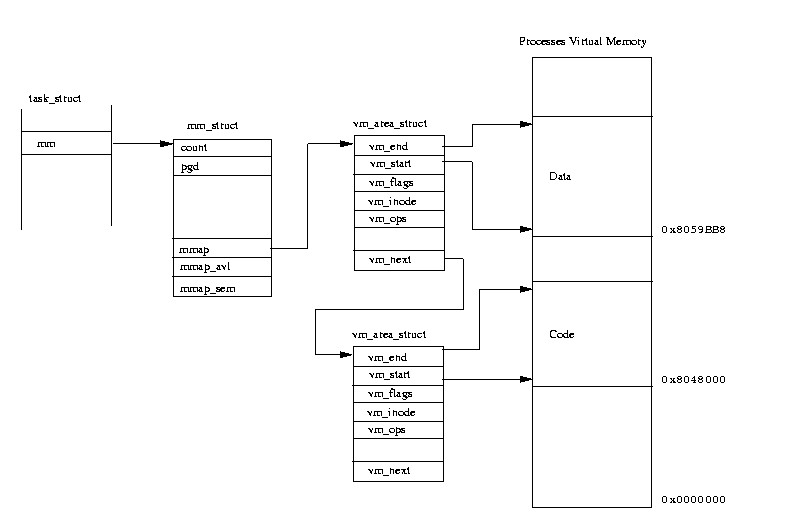
\includegraphics[width=\textwidth]{images/mm.jpg}
\caption{The structures used for virtual memory \url{https://www.tldp.org/LDP/tlk/kernel/processes.html}}
\label{img:mm}
\end{figure}
\verb|mmap| contains a list of virtual memory areas, which can contain the executable code, data, or code from shared libraries.
This list is actually organized in a binary tree, ordered by memory address, for faster access. These areas are allocated by the process as it runs, for example when it loads code of a shared library. Because it is virtual memory, each process has the illusion that it has the whole memory for itself, and that each time that it allocates memory it gets physically allocated. Such an approach would waste memory: what if the shared library is already loaded in RAM and used by other processes?

For this reason, Linux uses \textit{on-demand paging}. When a process allocates virtual memory, Linux does not actually reserve physical memory for the process. Instead, it describes the virtual memory by creating a new \verb|vm_area_struct| data structure. This is linked into the process's list of virtual memory. When the process attempts to write to a virtual address within that new virtual memory region then the system will page fault. Linux looks to see if the virtual address referenced is in the current process's virtual address space. If it is, Linux creates the appropriate \textit{page table entries} (PTEs) and allocates a physical page of memory for this process. The code or data may need to be brought into that physical page from the filesystem or from the swap disk. The process can then be restarted at the instruction that caused the page fault and, this time as the memory physically exists, it may continue.\cite{tlk}

\verb|mm_struct| has also a role in scheduling, because the \verb|mm|s of the two processes are switched upon context switch (Section TODO). The field \verb|mm| can also be set to \verb|NULL|: in this case the process is a kernel thread, free to use all the kernel space.

\paragraph{procfs}
The information contained in these structures can be accessed from outside the kernel with specific tools (covered in detail in Chapter \ref{chap:ftrace}). One approach to accomplish this it to use \verb|procfs|. In short, \verb|procfs| is a special filesystem that contains all the kernel information about processes, making it easy to access it from user space. For example, it is possible to gather scheduling information about process with pid 1196 by executing \verb|cat /proc/1196/schedstat|. This gives the following human-readable output:

\begin{verbatim}
tilda (1196, #threads: 3)
-------------------------------------------------------------------
se.exec_start                                :      26964101.112552
se.vruntime                                  :       2272975.687429
se.sum_exec_runtime                          :         10181.684621
se.nr_migrations                             :                11160
nr_switches                                  :                40529
nr_voluntary_switches                        :                40104
nr_involuntary_switches                      :                  425
se.load.weight                               :              1048576
se.avg.load_sum                              :              2453334
se.avg.util_sum                              :              2417183
se.avg.load_avg                              :                   45
se.avg.util_avg                              :                   45
se.avg.last_update_time                      :       26964101112552
policy                                       :                    0
prio                                         :                  120
clock-delta                                  :                   50
mm->numa_scan_seq                            :                    0
numa_pages_migrated                          :                    0
numa_preferred_nid                           :                   -1
total_numa_faults                            :                    0
current_node=0, numa_group_id=0
numa_faults node=0 task_private=0 task_shared=0 
group_private=0 group_shared=0
\end{verbatim}
Here, ``\verb|se|'' is the name of the field of type \verb|sched_entity| in \verb|task_struct|.

\paragraph{Red-black tree}
\label{sec:rb-tree}
The runnable tasks are stored inside a red-black tree, which allows more efficiency. A red-black tree is a type of self-balancing binary search tree: this means that the insertion and deletion operations will keep the height of the tree as small as possible. This characteristic is important because the cost of the most common functions (search, insertion and deletion) is proportional to the height of the tree.
As stated before, the task to run next is the one with the smallest vruntime. In a red-black tree, this corresponds to the task in the leftmost node. When picking the next task the tree is not traversed, instead, the leftmost node is cached in a dedicated variable in order to retrieve it faster.

\section{Time keeping}
\label{sec:timekeeping}
The kernel must keep track of time. The scheduler, for example, needs to know for how long a task has been running in order to know when to preempt it. There are many other functions that are time-driven, so it's important to understand how the system keeps track of the time.

To do this, the kernel requires an hardware timer. This timer can be implemented in different ways and there can be more timers in a system, but the general idea is the same: the timer sends an interrupt at a fixed frequency known by the kernel. This way, it's possible to get the time between two timer interrupts and perform periodic actions such as updating the system uptime. The period between two interrupts is a unit of measure called \textit{tick}, while the frequency is called \textit{tick rate}; this value is internally defined as the constant \texttt{HZ}. If the value of \texttt{HZ} is 100, there are 100 ticks per second, or one tick each 10 milliseconds.

\subsubsection{Choice of the tick rate}
Changing the frequency of the timer interrupt can have a large impact on the behavior of the system, so there are pros and cons to larger or smaller values of \texttt{HZ}.

%pros of larger HZ
A larger \texttt{HZ} means that the timer interrupt has a finer granularity: this means that all the timed events also have a higher resolution, which allows to improve their accuracy. As an example, let's consider process preemption: with an higher tick rate we can improve the accuracy and reduce the scheduling latency. Suppose that a process has 2 milliseconds left of its timeslice and the timer interrupt has just occurred. With an \texttt{HZ} of 100 the next interrupt will occur in 10 milliseconds, giving the process 8 extra milliseconds. This means that another task has to wait for more time in the runqueue, and this can be an issue for time-sensitive tasks. With a larger \texttt{HZ}, for example 1000, in the worst case scenario the latency is only 1 millisecond.

%cons of larger HZ
There is also a drawback to increasing the tick rate: the interrupt handler gets executed more often, and this results in less processor time for the tasks. The actual impact of the increased overhead is debatable and depends heavily on the speed of the processor.

%different values of HZ
The value of \texttt{HZ} depends on hardware and on the kernel configuration. On i386 \texttt{HZ} had a value of 100, with Linux version 2.6 the value was raised to 1000 and later was made a configurable parameter, with a default of 250. There were also introduced other, more accurate and \texttt{HZ}-independent, timers called \textit{high resolution timers} (HRT), making a high \texttt{HZ} less necessary. It is also possible to configure the kernel as \textit{tickless} (\verb|NO_HZ|): this means that the interrupt is no longer at fixed intervals, but it's dynamically scheduled as needed, which is helpful for power saving.

\subsubsection{Jiffies}
%What is jiffies
``\textit{Jiffies}'' is the number of ticks that have occurred since the system started. Every time that the interrupt handler is executed, the value of jiffies is increased by one. This means that with the value of \texttt{HZ}, and the value of jiffies, we can easily convert from seconds to jiffies by doing \verb|seconds * HZ| and from jiffies to seconds with \verb|jiffies / HZ|.
\begin{code}
// ./kernel/sched/sched.h
/*
 * Helpers for converting nanosecond timing to jiffy resolution
 */
#define NS_TO_JIFFIES(TIME) ((unsigned long)(TIME) / (NSEC_PER_SEC / HZ))
\end{code}

\paragraph{sched\_clock()}
\label{sched_clock}
An important function is \verb|sched_clock()|: it returns the system's uptime in nanoseconds. An architecture may provide an implementation, but if it is not provided, the system will use the jiffies counter to calculate the system's uptime.

The scheduler uses this function to determine the absolute, non-weighted, time that the current task has been running (\verb|se->runtime|). If the system uses the jiffies counter to determine this value, the maximum resolution of \verb|sched_clock()| depends on \texttt{HZ}. In this case the choice of \texttt{HZ} becomes more relevant.
The following is the default implementation of \verb|sched_clock()| when using only jiffies:
\begin{code}
unsigned long long __weak sched_clock(void)
{
	return (unsigned long long)(jiffies - INITIAL_JIFFIES)
					* (NSEC_PER_SEC / HZ);
}
\end{code}

\subsubsection{Timer interrupt handler}

The timer interrupt handler invokes other functions, some of which are architecture dependent. The other, architecture independent, timer functions are executed by \verb|tick_periodic()|, which is called by the handler.

\begin{code}
// ./kernel/time/tick-common.c
static void tick_periodic(int cpu)
{
	if (tick_do_timer_cpu == cpu) {
		write_seqlock(&jiffies_lock);

		/* Keep track of the next tick event */
		tick_next_period = ktime_add(tick_next_period, tick_period);

		do_timer(1);
		write_sequnlock(&jiffies_lock);
		update_wall_time();
	}

	update_process_times(user_mode(get_irq_regs()));
	profile_tick(CPU_PROFILING);
}
\end{code}
The two most important functions here are \verb|do_timer()| and \verb|update_process_times()|. The first one increments the value of jiffies and updates the load statistics for the system. The second updates various statistics and the runtime of the current task: if the task has finished its timeslice, it will prompt a reschedule. %TIF_NEED_RESCHED?

\begin{code}
// ./kernel/time/tick-common.c
/*
 * Must hold jiffies_lock
 */
void do_timer(unsigned long ticks)
{
	jiffies_64 += ticks;
	calc_global_load(ticks);
}
\end{code}

\subsubsection{update\_process\_times()}
This function updates the time that the current process has been running. The procedure changes if the process was running in user mode or in kernel mode. Remember that \verb|task_struct| has two different fields \verb|utime| and \verb|stime| to keep track of time spent in user space and in kernel space respectively. This function also invokes the \verb|scheduler_tick| function, which is the entry point that calls all the scheduler routines.

\begin{code}
// ./kernel/time/timer.c
/*
 * Called from the timer interrupt handler to charge one tick to the current
 * process.  user_tick is 1 if the tick is user time, 0 for system.
 */
void update_process_times(int user_tick)
{
	struct task_struct *p = current;

	/* Note: this timer irq context must be accounted for as well. */
	account_process_tick(p, user_tick);
	run_local_timers();
	rcu_check_callbacks(user_tick);
#ifdef CONFIG_IRQ_WORK
	if (in_irq())
		irq_work_tick();
#endif
	scheduler_tick();
	if (IS_ENABLED(CONFIG_POSIX_TIMERS))
		run_posix_cpu_timers(p);
}
\end{code}

\section{Scheduler routines}
There are essentially two ways of prompting a reschedule:
\begin{itemize}
    \item When the timeslice of the current process expires. When this occurs, the \verb|TIF_NEED_RESCHED|
    flag in the \verb|thread_info| structure of the current process is set, so the scheduler is
    invoked when the timer interrupt handler terminates.\cite{cesati} This rescheduling possibility is checked periodically, at each system tick.
    \item When a task is added to the runqueue. When it happens, the kernel checks whether its dynamic priority is
    greater than the priority of the currently running process. If it is, the execution of
    current is interrupted and the scheduler is invoked to select another process to run
    (usually the process that just became runnable).\cite{cesati} This rescheduling possibility is checked every time that a task is created or woken up.
\end{itemize}
The internal workings of these two procedures is illustrated, in order, in the two upcoming sections. There are other times in which a reschedule is prompted: indeed, \verb|schedule()| could be called like any other function, but this is done rarely in practice.

\subsection{Periodic reschedule}
We will now analyze in detail how scheduling works and the most important functions involved. In the last section, we saw how the system can perform periodic functions in order to measure time. From the entry point \verb|scheduler_tick()|, the subsequent calls can be traced with \verb|ftrace|: a function/event tracer embedded in the kernel.

The following script can trace function calls of any input kernel function. Function tracing with \verb|ftrace| is explained in detail in Chapter \ref{chap:ftrace}. For now, it is enough to know that this script simply sets \verb|ftrace| parameters before starting the trace. 
\begin{codebash}
#!/bin/bash
echo function_graph > /sys/kernel/debug/tracing/current_tracer
# removing noise to see just the actual function trace
# trace on cpu0 only (actually disables tracing on other cpus)
echo 1 > /sys/kernel/debug/tracing/tracing_cpumask 
# show comments on all exit points
echo funcgraph-tail > /sys/kernel/debug/tracing/trace_options 
# function to trace
echo $* > /sys/kernel/debug/tracing/set_graph_function
# clear previous trace
echo > /sys/kernel/debug/tracing/trace
sleep 3
cat /sys/kernel/debug/tracing/trace
\end{codebash}
%show trace starting from the timer interrupt, using function_graph tracer
With ``\verb|scheduler_tick|'' as input, this is a small piece of the output trace. Next, it is shown what's inside these functions.
\begin{Verbatim}
0)               |  scheduler_tick() {
0)   0.238 us    |    _raw_spin_lock();
0)   0.207 us    |    update_rq_clock.part.84();
0)               |    task_tick_fair() {
0)               |      update_curr() {
0)   0.167 us    |        update_min_vruntime();
0)   0.305 us    |        cpuacct_charge();
0)   3.652 us    |      } /* update_curr */
0)   0.219 us    |      __compute_runnable_contrib();
0)   0.159 us    |      __compute_runnable_contrib();
0)   0.114 us    |      intel_pstate_update_util();
0)   0.263 us    |      update_cfs_shares();
0)   0.178 us    |      hrtimer_active();
0) + 15.135 us   |    } /* task_tick_fair */
0)               |    cpu_load_update_active() {
0)   0.163 us    |      tick_nohz_tick_stopped();
0)               |      cpu_load_update() {
0)   0.178 us    |        sched_avg_update();
0)   1.927 us    |      } /* cpu_load_update */
0)   5.132 us    |    } /* cpu_load_update_active */
0)   0.148 us    |    calc_global_load_tick();
0)               |    trigger_load_balance() {
0)   0.400 us    |      idle_cpu();
0)   2.760 us    |    } /* trigger_load_balance */
0) + 33.332 us   |  } /* scheduler_tick */
\end{Verbatim}
In the following pieces of code, ``\verb|likely()|'' and ``\verb|unlikely()|'' are macros for \verb|gcc|'s built in branch prediction.
\begin{code}
// ./include/linux/compiler.h
#define likely(x)       __builtin_expect(!!(x), 1)
#define unlikely(x)     __builtin_expect(!!(x), 0)
\end{code}
These two macros are used in conditions. They indicate, respectively, that the condition is expected to be true or false. \verb|gcc| will then produce the correct assembly at compile time. If the guess is correct, less CPU cycles are used to choose the branch, but if it's not, the cycles are doubled. The double inversion (\verb|!!|) is to make sure the parameter is binary.

\subsubsection{scheduler\_tick}
As stated earlier, this function is called by the interrupt handler at every system tick.

\begin{code}
// ./kernel/sched/core.c
void scheduler_tick(void)
{
	int cpu = smp_processor_id();
	struct rq *rq = cpu_rq(cpu);
	struct task_struct *curr = rq->curr;
	struct rq_flags rf;

	sched_clock_tick();

	rq_lock(rq, &rf);

	update_rq_clock(rq);
	curr->sched_class->task_tick(rq, curr, 0);
	cpu_load_update_active(rq);
	calc_global_load_tick(rq);
	psi_task_tick(rq);

	rq_unlock(rq, &rf);

	perf_event_task_tick();

#ifdef CONFIG_SMP
	rq->idle_balance = idle_cpu(cpu);
	trigger_load_balance(rq);
#endif
}
\end{code}
The first important function here is \verb|sched_clock_tick()|. This function updates the per-CPU \verb|sched_clock_data| struct. To update this time, it uses the \verb|sched_clock()| function discussed earlier.

\verb|update_rq_clock()| updates the \verb|clock_task| field inside the runqueue of the current CPU (\verb|cpu_rq(cpu)|). This is used later by \verb|update_curr()|, a function that updates the \verb|task_struct| of the currently running process (stats, vruntime, runtime\dots).

Then, on line 14, \verb|task_tick()| is invoked for the current task to update its statistics. This action depends on the scheduling class that the current process is using. As shown in Section \ref{sec:sched_class}, \verb|sched_class| contains hooks to the correct functions for each scheduling class. Suppose that the current task has the fair class, then \verb|task_tick_fair()| would be executed on this line.

\subsubsection{task\_tick\_fair}

The runtime statistics for the current process are stored in the \verb|sched_entity| associated with it. The scheduler updates its parameters and then checks if the current task is to be rescheduled. 

\begin{code}
// ./kernel/sched/fair.c
static void task_tick_fair(struct rq *rq, struct task_struct *curr, int queued)
{
	struct cfs_rq *cfs_rq;
	struct sched_entity *se = &curr->se;

	for_each_sched_entity(se) {
		cfs_rq = cfs_rq_of(se);
		entity_tick(cfs_rq, se, queued);
	}

	if (static_branch_unlikely(&sched_numa_balancing))
		task_tick_numa(rq, curr);

	update_misfit_status(curr, rq);
}
\end{code}
This function fetches the \verb|sched_entity| of the current process. This is going to be a leaf of the hierarchy, and if the task isn't part of a group, it is also the root. Remember that the \verb|sched_entity| struct points to two runqueues: \verb|cfs_rq| and \verb|my_q|. The first is the runqueue on which the entity is scheduled, the second is the runqueue that belongs to that group. When the entity is a leaf, the second field is empty. 

For each entity in the hierarchy starting from the leaf, the function calls:
\begin{itemize}
    \item \verb|cfs_rq_of(se)|. This returns the runqueue on which the entity is scheduled. If the system is configured without group scheduling there is only one runqueue.
    
    \item \verb|entity_tick(cfs_rq, se, queued)|. This updates the statistics of that entity, then checks if it has finished its time and if another entity deserves to run. This means that:
    \begin{enumerate}
        \item If a process inside a group still deserves more time
        \item but the entire group has finished its time
        \item and another group deserves the CPU
    \end{enumerate}
    Then the task is preempted anyway. \verb|entity_tick()| also updates the load statistics used to balance the load between CPUs.
\end{itemize}

\subsubsection{entity\_tick}
\begin{code}
// ./kernel/sched/fair.c
static void
entity_tick(struct cfs_rq *cfs_rq, struct sched_entity *curr, int queued)
{
	/*
	 * Update run-time statistics of the 'current'.
	 */
	update_curr(cfs_rq);

	/*
	 * Ensure that runnable average is periodically updated.
	 */
	update_load_avg(cfs_rq, curr, UPDATE_TG);
	update_cfs_group(curr);

#ifdef CONFIG_SCHED_HRTICK
	/*
	 * queued ticks are scheduled to match the slice, so don't bother
	 * validating it and just reschedule.
	 */
	if (queued) {
		resched_curr(rq_of(cfs_rq));
		return;
	}
	/*
	 * don't let the period tick interfere with the hrtick preemption
	 */
	if (!sched_feat(DOUBLE_TICK) &&
			hrtimer_active(&rq_of(cfs_rq)->hrtick_timer))
		return;
#endif

	if (cfs_rq->nr_running > 1)
		check_preempt_tick(cfs_rq, curr);
}
\end{code}
\subsubsection{update\_curr}
\label{sec:update_curr}

The first part of \verb|entity_tick()|'s job, updating the runtime statistics, is done by \verb|update_curr()|. This function takes as argument only the runqueue on which the current task is running. From the runqueue, it gets the \verb|sched_entity| of the current task. It also gets the current time from the runqueue's clock, previously updated through \verb|update_rq_clock()|.

\label{trace:sched_stat_runtime}
\begin{code}
// ./kernel/sched/fair.c
static void update_curr(struct cfs_rq *cfs_rq)
{
	struct sched_entity *curr = cfs_rq->curr;
	u64 now = rq_clock_task(rq_of(cfs_rq));
	u64 delta_exec;

	if (unlikely(!curr))
		return;

	delta_exec = now - curr->exec_start;
	if (unlikely((s64)delta_exec <= 0))
		return;

	curr->exec_start = now;

	schedstat_set(curr->statistics.exec_max,
		      max(delta_exec, curr->statistics.exec_max));

	curr->sum_exec_runtime += delta_exec;
	schedstat_add(cfs_rq->exec_clock, delta_exec);

	curr->vruntime += calc_delta_fair(delta_exec, curr);
	update_min_vruntime(cfs_rq);

	if (entity_is_task(curr)) {
		struct task_struct *curtask = task_of(curr);

		trace_sched_stat_runtime(curtask, delta_exec, curr->vruntime);
		cgroup_account_cputime(curtask, delta_exec);
		account_group_exec_runtime(curtask, delta_exec);
	}

	account_cfs_rq_runtime(cfs_rq, delta_exec);
}
\end{code}
\verb|curr->exec_start| is the time at which the entity was selected by the scheduler to be executed. %pick_next_entity()->set_next_entity()->update_stats_curr_start()
We can calculate \verb|delta_exec|, the amount of time that the task has spent running, simply by subtracting \verb|exec_start| from the current time. \verb|exec_start| is then reset to the current time. \verb|delta_exec| is used to update the total \textbf{actual} runtime of the entity (\verb|sum_exec_runtime|). Other statistics are also updated, such as the longest execution so far (\verb|statistics.exec_max|).

The virtual runtime is the total runtime weighted. The weighted delta is calculated on line 22 by \verb|calc_delta_fair()|, and the virtual runtime is updated.
If the newly calculated vruntime is also the smallest in the runqueue, the field \verb|cfs_rq->min_vruntime()| is updated.
\verb|update_curr()| also triggers the trace event \verb|sched_stat_runtime|: this event signals when a process' virtual runtime is updated.

It is also possible that a group of tasks has a limit on the amount of CPU it can use. The function \verb|account_cfs_rq_runtime| is specific for groups. It updates \verb|cfs_rq->remaining_runtime|, where \verb|cfs_rq| is, again, the runqueue of the current group; then it triggers a reschedule if the remaining time reaches zero.

\subsubsection{calc\_delta\_fair and \_\_calc\_delta}
This function and its subfunction are a mere application of equation \ref{eq:vruntime}. Like the formula, this function weights the delta. \verb|__calc_delta| is where it's applied: it also takes the same parameters as the equation. 
\begin{code}
// ./kernel/sched/fair.c
/*
 * delta /= w
 */
static inline u64 calc_delta_fair(u64 delta, struct sched_entity *se)
{
	if (unlikely(se->load.weight != NICE_0_LOAD))
		delta = __calc_delta(delta, NICE_0_LOAD, &se->load);

	return delta;
}
\end{code}
\subsubsection{check\_preempt\_tick}

\verb|check_preempt_tick()| is called at the end of \verb|entity_tick()|, after all the fields of the current process have been updated with \verb|update_curr()|. Its job is to check if the current task has to be preempted. 
\begin{code}
// ./kernel/sched/fair.c
/*
 * Preempt the current task with a newly woken task if needed:
 */
static void
check_preempt_tick(struct cfs_rq *cfs_rq, struct sched_entity *curr)
{
	unsigned long ideal_runtime, delta_exec;
	struct sched_entity *se;
	s64 delta;

	ideal_runtime = sched_slice(cfs_rq, curr);
	delta_exec = curr->sum_exec_runtime - curr->prev_sum_exec_runtime;
	if (delta_exec > ideal_runtime) {
		resched_curr(rq_of(cfs_rq));
		/*
		 * The current task ran long enough, ensure it doesn't get
		 * re-elected due to buddy favours.
		 */
		clear_buddies(cfs_rq, curr);
		return;
	}

	/*
	 * Ensure that a task that missed wakeup preemption by a
	 * narrow margin doesn't have to wait for a full slice.
	 * This also mitigates buddy induced latencies under load.
	 */
	if (delta_exec < sysctl_sched_min_granularity)
		return;

	se = __pick_first_entity(cfs_rq);
	delta = curr->vruntime - se->vruntime;

	if (delta < 0)
		return;

	if (delta > ideal_runtime)
		resched_curr(rq_of(cfs_rq));
}
\end{code}
The first step is calculating \verb|ideal_runtime|. As the name suggests, this is the timeslice assigned to the task: remember that CFS's timeslice always varies dynamically.

If the task has run for more than the ideal runtime, the function \verb|resched_curr()| is called and it will cause the preemption of the task. The other way this function can trigger a reschedule, is if the difference between the virtual runtime of the current task and the smallest virtual runtime in the runqueue is bigger than the ideal runtime.

\paragraph{sched\_slice}
\begin{code}
/*
 * We calculate the wall-time slice from the period by taking a part
 * proportional to the weight.
 *
 * s = p*P[w/rw]
 */
static u64 sched_slice(struct cfs_rq *cfs_rq, struct sched_entity *se)
{
	u64 slice = __sched_period(cfs_rq->nr_running + !se->on_rq);

	for_each_sched_entity(se) {
		struct load_weight *load;
		struct load_weight lw;

		cfs_rq = cfs_rq_of(se);
		load = &cfs_rq->load;

		if (unlikely(!se->on_rq)) {
			lw = cfs_rq->load;

			update_load_add(&lw, se->load.weight);
			load = &lw;
		}
		slice = __calc_delta(slice, se->load.weight, load);
	}
	return slice;
}
\end{code}
\verb|sched_slice()| first calculates $target\_latency$ of equation \ref{eq:assigned_time}---also known as the \textit{scheduler period}. Remember that this value is defined as a period of time in which each task runs once, for at least \verb|sysctl_sched_min_granularity| nanoseconds. It is calculated through \verb|__sched_period()|.\label{sec:sched_period}
Here, two important scheduler tunables are used:
\begin{itemize}
    \item \verb|sysctl_sched_min_granularity| -- the minimum time a task is be allowed to run on a CPU before being preempted.
    \item \verb|sysctl_sched_latency| -- the default scheduler period.
\end{itemize}
\begin{code}
/*
 * The idea is to set a period in which each task runs once.
 *
 * When there are too many tasks (sched_nr_latency) we have to stretch
 * this period because otherwise the slices get too small.
 *
 * p = (nr <= nl) ? l : l*nr/nl
 */
static u64 __sched_period(unsigned long nr_running)
{
	if (unlikely(nr_running > sched_nr_latency))
		return nr_running * sysctl_sched_min_granularity;
	else
		return sysctl_sched_latency;
}
\end{code}
Lastly, the actual timeslice is calculated through \verb|__calc_delta()| on line 24: the result is the \verb|assigned_time| of equation \ref{eq:assigned_time}. Here, the first argument is the target latency, the second is the weight of the entity and the third is the total load of the current runqueue.

It may seem strange that \verb|__calc_delta()| is used to compute both the timeslice and vruntime (Equations \ref{eq:assigned_time} and \ref{eq:vruntime}), but the two formulas have the same structure, just with different arguments.

\paragraph{resched\_curr}\label{trace:wake_idle_without_ipi}
Finally, this function (called in \verb|check_preempt_tick()|) sets the \verb|TIF_NEED_RESCHED| flag, located in the flags field of the struct \verb|thread_info| (Section \ref{sec:thread_info}). 
This flag indicates that the current task needs to be rescheduled. When resuming the execution of a user process, the flag is checked and if it is set, the schedule function is called.

\subsection{Reschedule when adding a task to the runqueue}
A task can be added to the runqueue in 2 cases: when it is created, and when it is woken up. The reason why it's important to reschedule upon creation/wakeup is interactivity. If the newly added process has less weight than the running task, then it is scheduled. For example, if we pressed a button on a text editor, we expect its process to wake up and be rescheduled immediately in order to respond to the key press. In practice, the reschedule would often take place because the text editor's vruntime is very small. Moreover, after having responded to the key press, it will go back to sleep, keeping his vruntime to a minimum.
%CFS intuition here

\subsubsection{A new process is created}
When a process calls \verb|fork()| its \verb|task_struct| is duplicated and a new process is started. This is done by the \verb|_do_fork()| handler that also triggers the \verb|trace_sched_process_fork|\label{trace:sched_process_fork} event. It then calls \verb|wake_up_new_task()| that takes as argument the newly created \verb|task_struct|. 

This function sets the state of the task as \verb|TASK_RUNNING|, then, after initiating some values used for scheduling statistics, invokes \verb|activate_task()|. After the task has been activated and placed on the runqueue, \verb|wake_up_new_task| triggers the \verb|sched_wakeup_new| \label{trace:sched_wakeup_new} event. Lastly, this function calls \verb|check_preempt_curr()|, which will preempt the current task if another is more deserving. 

\paragraph{check\_preempt\_curr}\label{check_preempt_curr}
This function has a name that is very similar to\\ \verb|check_preept_tick|. It also has a similar function, but unlike \verb|check_preept_tick|, it is not periodic.
This function compares the newly created task with the one currently running. The first thing it has to check is the scheduling class: a task of a lower priority class cannot preempt one of an higher class. On the other hand, if the new task has an higher priority, the \verb|resched_curr()| function is called, causing a reschedule.
\begin{code}
void check_preempt_curr(struct rq *rq, struct task_struct *p, int flags)
{
	const struct sched_class *class;

	if (p->sched_class == rq->curr->sched_class) {
		rq->curr->sched_class->check_preempt_curr(rq, p, flags);
	} else {
		for_each_class(class) {
			if (class == rq->curr->sched_class)
				break;
			if (class == p->sched_class) {
				resched_curr(rq);
				break;
			}
		}
	}
	// ...
}
\end{code}
When the two tasks have the same scheduling class, the decision depends on the class, and the correct hook is invoked through \verb|sched_class|. If they use the \verb|fair_sched_class|, the \verb|check_preempt_wakeup()| function in \verb|fair.c| is called.

In this function, if the current task's policy is \verb|SCHED_IDLE| and the new task has a different policy, then the old task is preempted. Also, a batch or an idle task cannot preempt a non-idle task. If the tasks have the same policy, the virtual runtime of the current task is updated and then compared with the virtual runtime of the new task. This is done through this funciton:

\begin{code}
static int
wakeup_preempt_entity(struct sched_entity *curr, struct sched_entity *se)
{
	s64 gran, vdiff = curr->vruntime - se->vruntime;

	if (vdiff <= 0)
		return -1;

	gran = wakeup_gran(se);
	if (vdiff > gran)
		return 1;

	return 0;
}
\end{code}
If the current task has a smaller virtual runtime than the new one, the task is not preempted. Otherwise it is preempted if the difference between the virtual runtimes is big enough. This is done to avoid too frequent rescheduling. 

The scheduler has a tunable parameter called \verb|wakeup_granularity| that controls the minimum difference necessary to preempt the task (``big enough''). This value is not directly used, but instead, it's first weighted by the weight of the new task with \verb|calc_delta_fair()|. This is the same function used to calculate the virtual runtime. The new task is used, instead of the current one, because this penalizes tasks with smaller weights:
\begin{itemize}
    \item If the new task has a smaller weight than the current one, then the corresponding weighted granularity will be larger. This means that it is harder for the new task to preempt the current one.
    
    \item On the contrary, if the new task has a larger weight, it will be easier to preempt the current task. 
\end{itemize}

If the current task needs to be rescheduled, \verb|check_preempt_wakeup()| calls \verb|set_next_buddy()|, that tells to scheduler to favor the newly added task when choosing the next task. Finally, \verb|resched_curr()| is called.

\subsubsection{A task is woken up}

Waking up a process is similar to creating a new one: the task is first inserted into the runqueue and then the system checks if the currently running task needs to be rescheduled.

Before inserting the task into the runqueue, the \verb|sched_waking|\label{trace:sched_waking} event is triggered and the task's state is set to \verb|TASK_WAKING|. The task is then inserted into the runqueue by \verb|activate_task()|. Once it is on the runqueue, the \verb|task_struct->on_rq| field  is set to \verb|TASK_ON_RQ_QUEUED|. Finally, \verb|ttwu_do_wakeup()| is called, which checks if the current task can be preempted with \verb|check_preempt_curr()|; then it sets the task's state to \verb|TASK_RUNNING| and triggers the \verb|sched_wakeup|\label{trace:sched_wakeup} event.

\paragraph{enqueue\_task()}
Whether the task was just created or it was woken up from sleep, his \verb|task_struct| has to be added to the runqueue. This is done by the \verb|enqueue_task()| function. It takes as arguments a pointer \verb|rq| to the runqueue, a pointer \verb|p| to the \verb|task_struct| and an integer for the flags. It updates the \verb|cfs_rq| utilization statistics and invokes the \verb|enqueue_entity()| function that:
\begin{itemize}
    \item Calls \verb|update_curr()|, then adds \verb|cfs_rq->min_vruntime| to \verb|se->vruntime|. This is done because otherwise the new task would have a very small vruntime, which means huge boost compared to the other tasks. Note that the virtual runtime is decreased when dequeuing a task.
    \item Updates the load statistics of the entity and its group
    \item Calls \verb|__enqueue_entity()|, which inserts the entity of the \verb|task_struct| in the red-black tree representing the runqueue.
\end{itemize}
% TODO
% \subsubsection{schedule()}

% \subsubsection{context\_switch()}
